\documentclass{beamer}

\usepackage{pgfornament}

\usetheme{Berlin} 
%\usetheme{Darmstadt}
\useinnertheme{rounded}

\usefonttheme{serif}
\usecolortheme[RGB={0,10,100}]{structure} 
\setbeamertemplate{items}[circle] 
\setbeamertemplate{navigation symbols}{} 

\usepackage{amsmath, amsthm, amssymb}
\usepackage{amsfonts}
\usepackage{mathrsfs}

\usepackage{graphics}
\usepackage{graphicx}
\usepackage{hyperref}
\usepackage{multicol}


%\usepackage{textcomp}

\usepackage{float}

\usepackage{wrapfig}

\setbeamertemplate{blocks}[rounded][shadow=false]

% Required for inserting images
\usepackage{graphicx}

\usepackage[utf8]{inputenc}
\usepackage[T2A,T3,T1]{fontenc}

\usepackage[backref=true]{biblatex}
\addbibresource{ref.bib}

% https://latex.org/forum/viewtopic.php?t=20320
\DeclareSymbolFont{tipa}{T3}{cmr}{m}{n}
\DeclareMathAccent{\invbreve}{\mathalpha}{tipa}{16} 


\usepackage{amsmath, amsfonts, amssymb, bm}

\usepackage{yfonts}
\usepackage{mathrsfs}
\usepackage{pifont}
\usepackage{ifsym}
\usepackage{bbm}

\DeclareMathAlphabet\mathbfcal{OMS}{cmsy}{b}{n}
\usepackage{MnSymbol}
\usepackage{xcolor}
%\usepackage[colorlinks=true]{hyperref}
\usepackage{caption}
\usepackage{subcaption}
\usepackage{tabularx}
\usepackage{epigraph} 
\usepackage{algorithm}
\usepackage{todonotes}
%\usepackage{algpseudocode}



\definecolor{darkblue}{rgb}{0.0, 0.0, 0.55}
\definecolor{forestgreen}{rgb}{0.13, 0.55, 0.13}
\definecolor{darkteal}{rgb}{0.0, 0.24, 0.18}

\hypersetup{
  linkcolor=darkblue,
  urlcolor=darkteal,
  citecolor=forestgreen
}

\definecolor{w}{RGB}{231, 160, 76}
\definecolor{l}{RGB}{37, 84, 138}

\newcommand{\wbox}{\textcolor{w}{\blacksquare}}
\newcommand{\lbox}{\textcolor{l}{\blacksquare}}

\newcommand{\wb}{\square}
\newcommand{\bb}{\blacksquare}


%For diagrams
\usepackage{tikz-cd}
\usetikzlibrary{decorations.pathreplacing,fit,shapes.geometric}

% To solve the potential \Cross error in bbding
\usepackage{savesym} 

% For 5-star on dilation operator in Appendix D
\savesymbol{Cross}
\usepackage{bbding}
\restoresymbol{bb}{Cross} 



\usepackage{environ}

\usepackage{amsthm}
\usepackage{etoolbox} % Required for \AtBeginEnvironment and \AtEndEnvironment

\theoremstyle{definition}

%\newtheorem{definition}{Definition}[section]
\AtBeginEnvironment{definition}{%
  \pushQED{\qed}\renewcommand{\qedsymbol}{$\diamondsuit$}%
}
\AtEndEnvironment{definition}{\popQED}

%\newtheorem{theorem}{Theorem}[section]
\AtBeginEnvironment{theorem}{%
  \pushQED{\qed}\renewcommand{\qedsymbol}{$\spadesuit$}%
}
\AtEndEnvironment{theorem}{\popQED}

%\newtheorem{lemma}{Lemma}[section]
\AtBeginEnvironment{lemma}{%
  \pushQED{\qed}\renewcommand{\qedsymbol}{\rotatebox[origin=c]{180}{$\spadesuit$}}%
}
\AtEndEnvironment{lemma}{\popQED}

\newtheorem{conjecture}{Conjecture}[section]
\AtBeginEnvironment{conjecture}{%
  \pushQED{\qed}\renewcommand{\qedsymbol}{$\clubsuit$}%
}
\AtEndEnvironment{conjecture}{\popQED}

% Define the 'remark' environment with specific ending
\newtheorem*{remark}{Remark}
\AtBeginEnvironment{remark}{%
  \pushQED{\qed}\renewcommand{\qedsymbol}{$\triangle$}%
}
\AtEndEnvironment{remark}{\popQED}

\newtheorem{proofsketch}{ProofScetch}[section]
\AtBeginEnvironment{proofsketch}{%
  \pushQED{\qed}\renewcommand{\qedsymbol}{\rotatebox[origin=c]{180}{$\heartsuit$}}%
}
\AtEndEnvironment{lemma}{\popQED}

\renewcommand\qedsymbol{\textbf{Q.E.D.} \  $\heartsuit$}


% Definition of the Game Table environment

% Define a new counter
\newcounter{gametable}
\renewcommand{\thegametable}{\arabic{gametable}}

\newenvironment{gametable}[1][htb]
  {\refstepcounter{gametable}% Step the counter
   \begin{table}[#1]%
   \renewcommand{\tablename}{Game Table}% Rename table to Game Table
   \renewcommand{\thetable}{\arabic{gametable}}% Use separate numbering
  }
  {\end{table}}



\makeatletter
    \@ifdefinable{\PI}{\def\PI/{\mbox{Player 1}}}
    \@ifdefinable{\PII}{\def\PII/{\mbox{Player 2}}}
\makeatother

\newcommand{\G}[1]{$\textswab{Game}(#1)$}
\newcommand{\BG}[1]{$\textswab{BGame}(#1)$}
\newcommand{\SG}[1]{$\textswab{SGame}(#1)$}
\newcommand{\CG}[1]{$\textswab{CGame}(#1)$}

\newcommand{\InfG}[1]{$\overline{\textswab{Game}}(#1)$}
\newcommand{\InfBG}[1]{$\overline{\textswab{BGame}}(#1)$}
\newcommand{\InfSG}[1]{$\overline{\textswab{SGame}}(#1)$}
\newcommand{\InfCG}[1]{$\overline{\textswab{CGame}}(#1)$}


%Hbar
\usepackage{newunicodechar}

\makeatletter
\DeclareRobustCommand{\Hbar}{%
\text{
  \hmode@bgroup
  \vphantom{$H$}%
  \sbox\z@{$H$}%
  \ooalign{%
    $H$\cr
    \hidewidth
    \kern 0.1em % Adjust the horizontal position of the bar
    \vrule
      height \dimexpr 0.7\ht\z@+0.1ex\relax
      depth  -0.7\ht\z@
      width  0.8\wd\z@
    \hidewidth\cr
  }%
  \egroup
}
}
\makeatother

% Expectation
\newcommand{\E}{\mathbb{E}}

% Supp
\DeclareMathOperator\supp{supp}

% Rotated Clubsuit
\usepackage{rotating}

\newcommand{\rotatedclubsuit}{\mathbin{\text{\begin{sideways}\begin{sideways}$\clubsuit$\end{sideways}\end{sideways}}}}

% for Chinese, Japanese, and Korean characters
\usepackage{CJKutf8}

% for Ghost
\usepackage{halloweenmath}

% for \Pisces
\usepackage{marvosym}

% \mathds{1}
\usepackage{dsfont}

% for LoopedSquare
\DeclareRobustCommand{\loopedsquare}{\text{\raisebox{-.035em}{
\includegraphics[height=.6em]{img/logos/LoopedSquare.pdf}}}}

% for sampi
% from https://www.fileformat.info/info/unicode/char/03e0/index.htm
%\newcommand{\sampi}{\ensuremath{\includesvg[width=0.6em]{img/logos/sampi.svg}}}
\newcommand{\sampi}{\ensuremath{
\includegraphics[width=0.6em]{img/logos/sampi.pdf}}}

% for sha
% https://copyprogramming.com/howto/i-just-want-to-write-sha-without-ruining-everything
\newcommand\sh[1]{\ensuremath{\mathop{\text{\normalfont\fontencoding{T2A}\selectfont ш}}#1}}


% for the hexagon symbol
\newcommand{\hexacube}{
    
\begin{tikzpicture}[scale=0.15, baseline=-0.5ex]
        % Define the precise value for horizontal distance
        \pgfmathsetmacro{\hdist}{sqrt(3)/2}

        % Symmetric hexagon
        \draw (0,1) -- (\hdist,0.5) -- (\hdist,-0.5) -- (0,-1) -- (-\hdist,-0.5) -- (-\hdist,0.5) -- cycle;

        % Connect three non-consecutive vertices to the center
        \draw (0,0) -- (0,-1);
        \draw (0,0) -- (\hdist,0.5);
        \draw (0,0) -- (-\hdist,0.5);
    \end{tikzpicture}
}

\usepackage{caption}
\captionsetup[figure]{labelformat=empty}% redefines the caption setup of the figures environment in the beamer class.


\begin{document}

%\setbeamertemplate{background}{
\includegraphics[]{img/Background.png}} 


%\renewcommand{\thefootnote}{\fnsymbol{footnote}}


\title[Uncertainty and Game Theory]{Uncertainty and Game Theory \\ {\small \href{https://arxiv.org/abs/2503.01889}{Extended Equilibrium} \& \href{https://arxiv.org/abs/2402.15892}{Statistical Games}}}
\author{\href{https://konczer.github.io/}{József Konczer}}
\date{HUN-REN  \\ Rényi Institute of Mathematics
\\
\
\\
25 March 2025}

\begin{frame}
\titlepage
\end{frame}




%\begin{frame}{Overview}
%\end{frame}

\section{A fictional story}



\begin{frame}{Generals and the Weather }

    \begin{figure}
    \centering
        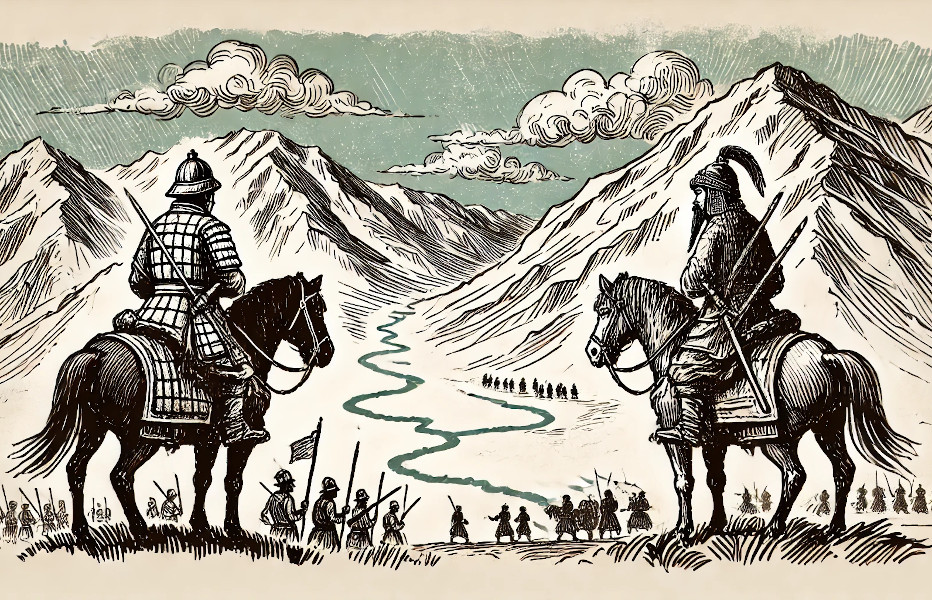
\includegraphics[width=0.85\textwidth]{img/GW.jpg}
        \caption{\small \centering (Illustartion generated by DALL·E at 2025. 03. 07. )}
    \end{figure}
    
\end{frame}

\begin{frame}{Generals and the Weather }

Imagine two generals, a ``Defender'' (Li) and an ``Attacker'' (Gar). To embed the story into a semi-historical context, one can picture the dilemmas of the generals and emperors from the Tang-Tibetan Wars in the 7th century. (The Himalayas or other mountains of Central Asia and the Tibetan Plateau could provide the mountain scene.) Li and Gar are preparing for battle near a mountainous region more than a thousand years ago – in an era when technology for reliable weather forecasting was not accessible.

The possible battlegrounds are new for both generals, but scouts identified two directions for the attack – an upper route in the hills and a lower route in a valley. In the hills, the ever-changing weather also plays a crucial role. By a sudden storm, it can wipe out a whole attacking army.
    
\end{frame}

\begin{frame}{Generals and the Weather }

Both generals can choose from two actions. Li can decide to defend the upper or the lower route, while Gar can decide to attack from the same two directions. The next day, the weather can be in two states; there can be a storm in the hills, or the weather can stay calm.

The winning and losing prospects depend on the actions of the generals and on the weather in the following way: If the weather is calm, then Li loses if he is attacked from an undefended direction, but the defense is always successful if both generals choose the same direction. In case of a storm, however, the attacking army would be lost if it dared the upper route. (On the lower route, in the valley, the weather does not change the outcome of a battle.)
    
\end{frame}

\begin{frame}{Generals and the Weather }

Assuming that no general has reliable knowledge about the weather or can reliably associate a probability distribution to it – and their lack of information is common knowledge – what strategy should the generals follow? (The generals are capable of randomization – methods such as divinations of various kinds were used from prehistory to make randomized actions.)
    
\end{frame}

\section{Games with Uncertainty}




\begin{frame}{}

\begin{definition}[Games with uncertainty]
\label{def:GameWithUncertainty}
A (finite, $N$-person, non-cooperative) game with (global) uncertainty is a tuple $\langle N, \underline{\mathcal{A}}, \Theta, \underline{U} \rangle$, where:

\begin{itemize}
    \item $N \in \mathbb{N}$ is the number of players;
    \item $\underline{\mathcal{A}} = (\mathcal{A}_1,\dots,\mathcal{A}_N)$ is the action set profile of the players, where all $\mathcal{A}_i$ are finite sets;
    \item $\Theta$ is a finite set of the globally unknown parameter or state. (Global uncertainty means that no player has credible side-information about it's value, and this is common knowledge);
    \item $\underline{U} = (U_1,\dots,U_N)$ is the set of subjective, action and parameter-dependent utility functions taking real values: $U_i : \underline{\mathcal{A}} \times \Theta \mapsto \mathbb{R}$.
\end{itemize}
    
\end{definition}

\end{frame}


\begin{frame}{Extended strategy}

    \begin{equation}
        \sigma_i \in \Delta(\mathcal{A}_i), \quad \pi_i \in \Delta(\Theta)
    \end{equation}

\begin{equation}
        \underline{\rho} = ( \underline{\sigma}; \underline{\pi} )
    \end{equation}

    
    \begin{equation}
        \underline{\rho} \in 
        \mathcal{R} :=
        \mathcal{S} \times \mathcal{P} =
        \left ( \bigtimes_{i=1}^N \Delta(\mathcal{A}_i) \right ) \times
        \left ( \Delta(\Theta) \right )^N
    \end{equation}

    
\end{frame}

\begin{frame}{Regret}

First definition:

    \begin{equation}
    R_i(\underline{a};\theta | \underline{\sigma}) = 
    \max_{c_i \in \mathcal{A}_i} 
    \left ( 
    \sum_{\underline{b} \in \underline{\mathcal{A}}} U_i(\underline{b}^{[i] \leftarrow c_i};\theta) \ \Pi(\underline{b}|\underline{\sigma})
    \right )
    -U_i(\underline{a};\theta)
\end{equation}

Alternative definition:

    \begin{equation}
    \label{defeq:EUMatrix}
        \mathrm{EU}_i(a_i;\theta | \underline{\sigma}) = 
        \sum_{\underline{b} \in \underline{\mathcal{A}}} U_i(\underline{b}^{[i] \leftarrow a_i};\theta) \ \Pi(\underline{b}|\underline{\sigma})
    \end{equation}

        \begin{equation}
    \label{eq:RegretMatrix}
        \mathrm{ER}_i(a_i;\theta | \underline{\sigma}) =
        \max_{c_i \in \mathcal{A}_i} \left ( \mathrm{EU}_i(c_i;\theta | \underline{\sigma}) \right ) - \mathrm{EU}_i(a_i;\theta | \underline{\sigma})
    \end{equation}
    
\end{frame}

\begin{frame}{Extended Equilibrium}

    \begin{definition}[Extended Equilibrium]
\label{def:ExEq}
We call a complete strategy profile $\underline{\rho}^* = (\underline{\sigma}^*;\underline{\pi}^*) \in \mathcal{R}$ an extended equilibrium if it fulfils the following set of inequalities:

    \begin{equation}
    \label{defeq:ExtendedEquilibriumEU}
        \forall i, \forall a_i \in \mathcal{A}_i, \  \mathrm{EU}_i(\underline{\sigma}^*;\underline{\pi}^*) \ge \mathrm{EU}_i(a_i | \underline{\sigma}^*;\underline{\pi}^*)
    \end{equation}
    \begin{equation}
    \label{defeq:ExtendedEquilibriumER}
        \forall i, \forall \theta \in \Theta, \  \mathrm{ER}_i(\underline{\sigma}^*;\underline{\pi}^*) \ge \mathrm{ER}_i(\theta | \underline{\sigma}^*;\underline{\pi}^*)
    \end{equation}

\end{definition}
    
\end{frame}

\begin{frame}{}

Extended equilibrium of the $\mathcal{GW}$ game:

\begin{equation}
    \sigma_1^* = (p, \bar{p}), \quad
    \sigma_2^* = (q, \bar{q})
\end{equation}

\begin{equation}
    \pi_1^* = (P, \bar{P}), \quad
    \pi_2^* = (Q, \bar{Q})
\end{equation}

With the parameters:
\begin{table}[H]
    \centering
    \tiny
    \renewcommand{\arraystretch}{1.5}
    \begin{tabular}{|c|c|c||c|c|c|}
        \hline
        \multicolumn{3}{|c||}{\textbf{Parameters ($x$)}} & \multicolumn{3}{c|}{\textbf{Complements ($\bar{x} = 1-x$)}} \\
        \hline
        \textbf{Variable} & \textbf{Exact expr.} & \textbf{Num. approx.} & \textbf{Variable} & \textbf{Exact expr.} & \textbf{Num. approx.} \\
        \hline
        $p$ & $1-1/\sqrt{2}$ & 0.293 & $\bar{p}$ & $1/\sqrt{2}$ & 0.707 \\
        \hline
        $q$ & $2-\sqrt{2}$ & 0.586 & $\bar{q}$ & $\sqrt{2} - 1$ & 0.414 \\
        \hline
        $P$ & $1/\sqrt{2}$ & 0.707 & $\bar{P}$ & $1-1/\sqrt{2}$ & 0.293 \\
        \hline
        $Q$ & $\sqrt{2} - 1$ & 0.414 & $\bar{Q}$ & $2-\sqrt{2}$ & 0.586 \\
        \hline
    \end{tabular}
    %\caption{Exact values and numerical approximations of the equilibrium parameters and their complements for the ``Generals and the weather'' ($\mathcal{GW}$) game's extended equilibrium.}
    \label{tab:variables}
\end{table}

\end{frame}

\section{Existence}

\begin{frame}{Auxiliary map $\Upsilon$}

We define a continuous auxiliary map $\Upsilon : \mathcal{R} \mapsto \mathcal{R}$ by first introducing the functions $\varphi_{i,a_i}(.;.)$ and $\psi_{i,\theta}(.;.)$:

    \begin{equation}
    \label{eq:varphiDef}
        \varphi_{i,a_i}(\underline{\sigma};\underline{\pi}) = 
        \mathrm{ReLU} 
        \left (
        \mathrm{EU_i}(a_i|\underline{\sigma};\underline{\pi})
        -
        \mathrm{EU_i}(\underline{\sigma};\underline{\pi})
        \right )
    \end{equation}

    \begin{equation}
    \label{eq:psiDef}
        \psi_{i,\theta}(\underline{\sigma};\underline{\pi}) = 
        \mathrm{ReLU} 
        \left (
        \mathrm{ER}_i(\theta | \underline{\sigma};\underline{\pi})
        -
        \mathrm{ER}_i(\underline{\sigma};\underline{\pi})
        \right )
    \end{equation}
    
\end{frame}


\begin{frame}{Auxiliary map $\Upsilon$}

Then by introducing the mappings $\Phi(.;.)$ and $\Psi(.;.)$

    \begin{equation}
        \underline{\sigma}' = \Phi(\underline{\sigma};\underline{\pi})
        \iff
        \sigma_i'(a_i) = \frac{\sigma_i(a_i) + \varphi_{i,a_i}(\underline{\sigma};\underline{\pi})}{1 + \sum_{b_i \in \mathcal{A}_i} \varphi_{i,b_i}(\underline{\sigma};\underline{\pi})} 
    \end{equation}

    \begin{equation}
        \underline{\pi}' = \Psi(\underline{\sigma};\underline{\pi})
        \iff
        \pi'_i(\theta) = \frac{\pi_i(\theta) + \psi_{i,\theta}(\underline{\sigma};\underline{\pi})}{1 + \sum_{\chi \in \Theta} \psi_{i,\chi}(\underline{\sigma};\underline{\pi})} 
    \end{equation}

    And finally, by combining these maps:
    
    \begin{equation}
        \Upsilon(\underline{\rho})
        =
        \Upsilon((\underline{\sigma};\underline{\pi}))
        =
        (\Phi(\underline{\sigma};\underline{\pi}); \Psi(\underline{\sigma};\underline{\pi})) 
        =
        (\underline{\sigma}';\underline{\pi}') 
        =
        \underline{\rho}'
    \end{equation}
    
\end{frame}

\begin{frame}{Fixed point Lemma}

The simple but crucial observation is that the defined auxiliary map is a continuous self-map of complete strategy profiles. (All $\varphi_{i,a_i}$ and $\psi_{i,\theta}$ are non-negative, and the normalization in the definition of $\Phi$ and $\Psi$ ensures that all $\sigma_i'$ and $\pi_i'$ are proper probability distributions):

\begin{equation}
    \Upsilon \in C^0(\mathcal{R},\mathcal{R})
\end{equation}

Therefore, based on Brouwer fixed-point theorem there exists a fixed point:


    \begin{equation}
    \exists \underline{\rho}^* \in \mathcal{R}, \quad \Upsilon(\underline{\rho}^*) = \underline{\rho}^* 
    \end{equation}
    
\end{frame}

\begin{frame}{Equivalence of Extended Equilibrium and Fixed points}

    \begin{theorem}[Equivalence of Extended Equilibrium and Fixed points]
\label{thm:Equivalence}
A complete strategy profile is an extended equilibrium if and only if it is a fixed point of the $\Upsilon : \mathcal{R} \mapsto \mathcal{R}$ map. Formally:

    \begin{equation}
        \Upsilon(\underline{\rho}^*) = \underline{\rho}^* \iff
        \underline{\rho}^*=(\underline{\sigma}^*;\underline{\pi}^*) \text { is an extended equilibrium}
    \end{equation}
\end{theorem}
    
\end{frame}

\begin{frame}{Equivalence of Extended Equilibrium and Fixed points}

    \begin{proof}

We can prove both directions of the statement.

\

{\bf Extended Equilibrium $\implies$ Fixed point:}
(Easy)


\

{\bf Fixed point $\implies$ Extended equilibrium:} (Tedious but straightforward to check.)

\

See details in \href{https://arxiv.org/abs/2503.01889}{arXiv:2503.01889}

\end{proof}
    
\end{frame}

\begin{frame}{Existence of Extended Equilibrium}

    \begin{proof}
{\bf Existence of Extended Equilibrium:}
The previous lemma guarantees the existence of a fixed point of the auxiliary mapping $\Upsilon : \mathcal{R} \mapsto \mathcal{R}$;
while the previous theorem assures that a fixed point of $\Upsilon(.)$ is necessarily also a complete strategy profile in extended equilibrium.

This completes the proof.
    
\end{proof}
    
\end{frame}

\section{No Fictional Faith}

\begin{frame}{}

\begin{theorem}[No Fictional Faith]
\label{thm:NoFictionalFaith}
    For any player $i$, a ``pure prior'', $\pi_i^{\eta}(\theta) = \delta_{\eta,\theta}$ (where $\delta$ stands for Kronecker delta) can be part of an extended equilibrium $(\underline{\sigma}^*, \underline{\pi}^*)$ only if the parameter is ``irrelevant'' for the $i$-th player, i.e. in the equilibrium there is an action (or actions) that is a best response -- there is no alternative action yielding higher expected utility -- regardless of the unknown parameter. 

    \
    
    If a ``pure prior'' appears in an equilibrium solution for the $i$-th player, then  $\pi_i^*$ is totally degenerate. Any prior $\pi'_i \in \Delta(\Theta)$ could be substituted to the subjective equilibrium prior of the $i$-th player $\pi_i^{\eta}$, preserving the conditions for the extended equilibrium. Therefore, a continuum set of extended equilibria solutions exists in this case.

\end{theorem}

    
\end{frame}

\begin{frame}{}

    \begin{remark}
    The ``No Fictional Faith'' theorem ensures that the equilibrium priors satisfy a weakened regularity condition. In Bayesian inference,
    the so-called Cromwell's rule -- also known as the regularity requirement -- suggests not to use a prior which associates $0$ or $1$ to specific events.
    In extended equilibrium -- if the parameter is not irrelevant to a player -- the subjective equilibrium prior will not associate probability $1$ to any specific parameter, therefore automatically satisfying the second half of Cromwell's rule --in cases where the parameter matters.

    (If the unknown parameter can take only two values, i.e. $|\Theta|=2$, the theorem guarantees the strong form of regularity.)
    
\end{remark}
\end{frame}

\begin{frame}{Irregular emergent subjective prior}
    
    Consider the following simple single-player game with uncertainty:

    The player has two possible actions: $\mathcal{A_1} = \{\mathrm{U},\mathrm{D}\}$; while the uncertain parameter can be in three states: $\Theta=\{\mathrm{L},\mathrm{C},\mathrm{R}\}$.
    The utility function -- in this case representable by a single matrix -- is given below:

    \begin{equation}
        U_1(.;.) = 
        \begin{bmatrix}
            1 & 0 & 0 \\
            0 & 0 & 1
        \end{bmatrix}
    \end{equation}

    In this simple case, we can easily construct the effective regret matrix:

    \begin{equation}
        R_1(.;.) = 
        \begin{bmatrix}
            0 & 0 & 1 \\
            1 & 0 & 0
        \end{bmatrix}
    \end{equation}

\end{frame}

\begin{frame}{Irregular emergent subjective prior}

    It is easy to see and verify that this game has one unique extended equilibrium, with the following strategy and emergent subjective prior pair:

    \begin{equation}
        \sigma_1^* = (1/2,1/2), \quad \pi_1^* = (1/2, 0, 1/2)
    \end{equation}

    The previous simple example demonstrates that in some cases, zero probability might appear in the equilibrium prior.

    \
    
    However, the possibility of making an observation and collecting data leads to an extended game with a richer action set. In these extended games, new priors have to be obtained, which opens up the possibility to avoid the problem of ruling out potential states à priori. (``Convincing Signals Theorem'')

\end{frame}

\section{Related Frameworks}

\begin{frame}{}

{\bf Games with chance nodes:}
The introduction of a
``Chance player'' -- often called ``Nature'' --, which is assumed to make a ``chance move'' with predefined probabilities $p_\theta$.

\

{\bf Bayesian games:}
Also known as Harsányi games, which introduces ``types'' for the players and a commonly known prior on these types. Formally a Bayesian game is a tuple: $\langle N, \underline{\mathcal{A}}, \underline{T}, \underline{U}, \pi_c \rangle$ where $U_i : \underline{\mathcal{A}} \times \underline{T} \to \mathbb{R}$ and $\pi_c \in \Delta(\underline{T})$.
    
\end{frame}

\begin{frame}{}

{\bf Bayesian games with inconsistent beliefs:}
In this -- more general but less common -- framework, one needs to specify not only one common prior for the types but a set of priors or beliefs $\underline{\pi}$.
One can define a -- generalized -- Bayesian equilibrium in games with incomplete information, which gives the same real equilibrium strategies $\underline{\sigma}^*$ of the extended equilibrium if the set of beliefs happens to be the equilibrium priors, i.e. $\underline{\pi} = \underline{\pi}^*$.

\ 

Therefore, the concept of extended equilibrium can be viewed as a prior selection mechanism for general Bayesian games with inconsistent beliefs.
    
\end{frame}

\section{Future work}




\begin{frame}[shrink=15]{Future work and extension, calls for Collaboration}

    \begin{columns}

\begin{column}{0.7\textwidth}
            
\begin{itemize}
    \item Assumptions about the unknown ($\mathghost$ vs. \hexacube{})
    \item Target of the Inference
    \begin{itemize}
        \item ``Platonian'' Inference (Inferential risk)
        \item ``Aristotelian'' Inference (Predictive risk)
        \item Data compression
        \item General: distinct Target and Data spaces
    \end{itemize}
    \item Correspondence with Bayesians and Frequentists
    \item Effective approximative numerical methods (Blahut–Arimoto algorithm)
    \item Generalizing Game Theory with a player representing uncertainty $\checkmark$
    \item Using the concept in Reinforcement Learning
    \item Foundations of Statistical Physics
    \item Quantum metrology
    \item Universal Inductive Inference
    \item \dots
\end{itemize}

        \end{column}

% Column 2    
\begin{column}{0.3\textwidth}
    \begin{figure}
    \centering
        
\includegraphics[width=0.9\textwidth]{img/logos/SagradaFamilia.pdf}
        \caption{\small \centering  \href{https://boutique.arte.tv/detail/sagrada-familia-le-defi-de-gaudi}{La Sagrada Família}, Antoni Gaudí: ``My client is in no hurry''.}
    \end{figure}
\end{column}
        

\end{columns}

\end{frame}

\begin{frame}{}

\centering \Huge
  {Thank you for your attention!}

    \vspace{0.85 cm}
    
  \pgfornament[height=0.85cm]{74}

    \vspace{0.85 cm}

    {\large
  \href{mailto:konczer.j@gmail.com}{konczer.j@gmail.com},
        \href{https://konczer.github.io/}{konczer.github.io}
        
        \vspace{0.3 cm}
        
        \href{https://arxiv.org/abs/2503.01889}{arXiv:2503.01889}
        
        \href{https://www.alphaxiv.org/abs/2503.01889}{alphaXiv:2503.01889}

        \href{https://github.com/Konczer/UncertaintyTheory/tree/main/ExtendedEqilibrium}{GitHub}
     }   
  
\end{frame}

\begin{frame}{}

\begin{figure}[H]
    \centering
    
\includegraphics[width=0.7\textwidth]{img/QuestioningMind.png}
\end{figure}

\end{frame}


\end{document}